
%%%%%%%%%%%%%%%%%%%%%%%%%%%%%%%%%%%%%%%%%%%%%%%%%%%%%%%%%%%%%%%%%%%%%%%%%%%
%
% Plantilla para un artculo en LaTeX en espaol.
%
%%%%%%%%%%%%%%%%%%%%%%%%%%%%%%%%%%%%%%%%%%%%%%%%%%%%%%%%%%%%%%%%%%%%%%%%%%%

\documentclass[11pt,twoside]{report}

% Esto es para poder escribir acentos directamente:
%\usepackage[latin1]{inputenc}
\usepackage[utf8]{inputenc}
\usepackage{makeidx}
\usepackage{multirow}
\usepackage{titlesec}
\usepackage{sectsty}
\usepackage{fncychap}
\usepackage{color}

% Esto es para que el LaTeX sepa que el texto est en espaol:
\usepackage[spanish]{babel}
\usepackage[right=3cm,left=3cm,top=2.5cm,bottom=2.5cm,headsep=1cm,footskip=2cm]{geometry}
\usepackage{graphicx}
% Paquetes de la AMS:
\usepackage{amsmath, amsthm, amsfonts}

%\pagestyle{headings}
\pagestyle{myheadings}
\markboth{Informe Semanal de Actividades Realizadas}{Informe Semanal de Actividades Realizadas}
\begin{document}
\title{\color{red}Informe Semanal de Actvividades Realizadas}
\author{Nombre: Arturo Veras\\ 
Supervisor: Claudio Torres\\
Empresa: CCTAVAL\\
Tipo de Práctica: Profesional}
%\date{\color{green}December 2005}
\maketitle
%\setlength{\unitlength}{1 cm} %Especificar unidad de trabajo
\thispagestyle{empty}
\begin{picture}(0,1.5)
\put(0,0){
\includegraphics[width=2.7cm,height=2cm]{utfsm.jpg}}
\put(13,0){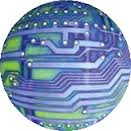
\includegraphics[width=2cm,height=2cm]{elo.jpg}}
\end{picture}
\\
\\
\begin{center}
\textbf{{\LARGE Universidad Técnica Federico Santa María}\\[0.5cm]
{\LARGE Departamento de Electrónica}}\\[4.25cm]
{\Large Informe de Práctica}\\[2.3cm]
{\LARGE \textbf{Centro Cient\'ifico Tecnol\'ogico de Valpara\'iso}}\\[3.5cm]
{\large Arturo Veras Olivos}\\[2cm]
Valparaiso - \today
\\
 {\large Versión 2.5}
\end{center}

%\newpage
%\tableofcontents
%\listoffigures % to produce list of figures
%\listoftables % to produce list of tables
%\newpage
\section*{IFORME SEMANAL DE ACTIVIDADES REALIZADAS}
\subsection*{Semana 1,  del 13/01/14 al 17/01/14}


The main idea is to connect the GT640 PCIe 3.0 16x interface to one of the RPi (Raspberry Pi) interfaces. The RPi has a GPIO and USB 2.0 port available that we are going to use for this purpose.

1.startKIT



startKIT is a low-cost development board for the configurable xCORE multicore microcontroller products from XMOS. It’s easy to use and provides lots of advanced features on a small, extremely low cost platform.

xCORE lets software-configure the interfaces that you need for your system; so with startKIT you can configure the board to your match your exact requirements. Its 500MIPS xCORE multicore microcontroller has eight 32bit logical cores that perform deterministically, making startKIT an ideal platform for functions ranging from robotics and motion control to networking and digital audio.

startKIT also connects easily to the Raspberry Pi, allowing you to add real-time I/O and communication features, and to try out advanced applications for xCORE. (more details in the startKIT Hardware Manual)

The block diagram of the solution is:

startKIT diagram

2. MCS9901-CC Chip

MCS9901CV-CC is a single lane multifunction PCI express to I/O controller. Some important features:

PCI Express.
Single-lane (X1) PCI Express End-point Controller with integrated PHY.
Four USB 2.0 Host Ports with on-chip transceivers, can handle High-speed (480Mbps), Full-speed (12Mbps) and Low-speed (1.5Mbps) transactions.
One of the USB 2.0 Host Port can support OTG feature. We leave this as last option because because it has high labor demand. If we want to implement this solution we need to develop the board bridge controller and the driver. Next day we are going to evaluate the ideas. The block diagram of the solution is:
MCS9990

January Thursday 16

We discard the startKIT because the board only has the PCIe driver for sliceCARD add-on boards, to connect the GPU have to program the controller and the GPIO RPi controller. So the startKIT only acts as hardware interface between PCIe and GPIOs, not a smart solution. Another potentially solution is:

PE4L-PM060A
:wq



The PE4L-PM060A is a PCIe Adapter. The PE4L is designed for Notebook PCs that converts PCI Express 1X add-on Card to ExpressCard or mPCIe connecter or PCI Express slot. As PCI Express x1 connector is edge-free / multi-lane, x4, x8 and x16 PCIe Cards are also available. This adapter allows you to use your existing PCI-E 1X Card in the notebook PC or Desktop PC for test. or AD-DC12V adapter). The RPi doesn't have a mPCIe interface so this adapter would be an option in the case of changing the RPi for another embedded system with MPCIe interface.

January Friday 17

We discard the PE4L-PM060A, this adapter does not solve the problem but is a good way to implement a power supply for the GPU, also if we have a card with mPCI.

We complete discard the RPi's GPIO ports because the speed is of the order of hundreds of KHz, the PCIe runs at the order of GHz. The low frequency of the GPIO coupled with the coding overhead for each pin it would be impossible to bit bang the Pi fast enought.
\subsection*{Semana 2, del 20/01/14 al 24/01/14}


We found a new device that enable forward and reverse bridging, the USB2380 is a PCI Express Gen 1 (2.5Gbps) to USB 2.0 Hi-Speed Peripheral Controller. It features one PCI Express Gen 1 x1 port and one USB 2.0 Hi-Speed client port. The USB 2380 provides 480Mbps bandwidth between the PCI Express Gen 1 bus and the USB 2.0 Hi-Speed bus. The controller can easily add a USB 2.0 client port to an existing PCI Express system. The USB 2380's standard PCI Express interface provides a x1 upstream port to connect directly to any PCI Express downstream port for maximum performance of the product. (more details in USB2380).

In theory this is what we need but we have this problems.

Does not have the price, so we have to wait until the vendor respond the email and we need a solution in short period of time.
The firmware is available to configure the USB 2380 to resemble a standard USB class device (like a printer or mass storage device) for which no USB host drivers will need to be written. For custom applications, firmware APIs are provided to abstract the USB transactions to reads and writes. And we do not know if this is opensource if we want to replicate.
With this product have been built a board which can be connected to a laptop, but are not sure if we can acquire this board in time.
Recall that USB 2380 do not provide power supply for GT640, the ATX power supply must be use.
January Tuesday 21

We recall the lastest option of implementation, the PCIe to USB Host Controller chipset.

MCS9990 – PCIe to 4-Port USB 2.0 Host Controller.

USB 2380.

The GT640 has a PCIe 3.0 16x interface, the host controllers support PCIe 1.1. In PCIe there is no problems with the connectivity with older versions. To connect the GT640 we need a PCIe 1x to 16x Powered Flexible Riser. In theory we have all we need to build a prototype that does the job. The next question is if the GT640 is going to be recognized by the RPi, there is driver support for this application? can we use the existing legacy drivers or we have to implement a new one?

In the meanwhile we are in contacts with the vendors to to see what they say about the feasibility of the project.

January Wednesday 22

Some of the vendors respond to our emails but the did't understand the requirements that we need. We explained and still we are waiting for the response.

We are studying MCS9990. There is an schematic circuit to make the board, but this is not what we need. Therefore we need to make a deep study of PCIe protocol and the MCS9990 chip to develop the PCIe to USB 2.0 adapter. This option is out of discussion because the time consuming of developing time is very high.

In conclusion any attempt to create an interface using a chip is discarded.

January Thursday 23

The SBC-A510 Single Board Computer. is a mini-ATX compliant, single board computer. Important features:

Single board computer implemented by the combination of a CM-A510 module and a SB-A510 baseboard. Mini-ATX form factor.
1GB DDR3
PCI Express and PCI extension interfaces
The price for 1k unit: USD $65. For 1 quantity 2.5*$65 = USD $163
January Friday 24

We couldn't find a definitely solution to the problem. This is the summary so far:

Found a USB 2380 board that can we use but the vendor did not contact us yet.
Use the PE4L-PM060A in the case of acquiring a board with the mPCIe.
Completely ruled out the solution to implement the MCS9990 chip or similar, not a feasible solution.
The project will take another tack. Since we can not, for the moment, to find a solution to connect the RPI to a PCI card, the new approach will be to seek ways to connect the GPU to some device that that we can transfer data through an USB port. The options we have high to low priority.

Development boards with PCIe slot that we can buy this week or soon.
mPCIe to PCIe adapter so we can use the development board that we already have.
Build a cheap computer to use as PCIe interface.
Finally we decided to use the USB port to communicate with the GPU to make a Plug and Play device. There can be another ideas like use the Ethernet port but the USB is going to be the main work. So, we need to find solutions to the problem of connecting the Host PC to the RPi or some other device which in turn will be connected to the GPU.
\subsection*{Semana 3, del 27/01/14 al 31/01/14}
\subsection*{Semana , del 03/02/14 al 07/02/14}



\end{document}
